\section{Auswertung}
\label{sec:Auswertung}

\subsection{Vorbereitung}

Für die Auswertung der beiden Versuchsteile, ist es nötig, die Fourierkoeffizienten der verschiedenen
Spannungsfunktionen (Sägezahn, Rechteck und Dreieck) erst theoretisch zu berechnen,
um diese dann mit den experimentell bestimmten vergleichen zu können. Dazu werden die Funktionsparametriesierungen
möglichst so gewählt, dass sie gerade oder ungerade sind und somit jeweils $b_k$ oder $a_k$ für alle $k$ verschwinden. \\

Für die Sägezahnspannung ergeben sich die Fourierkoeffizienten

\begin{align*}
    a_\text{k} &= 0 \\
    b_\text{k} &= - \frac{1}{2k} + \frac{1}{k}
\end{align*}

und nach \eqref{eqn:Entwicklung} die Fourierreihe

\begin{equation*}
    f(t) = \sum^\infty_{k = 1} \left( \left( - \frac{1}{2k} + \frac{1}{k} \right) \; \text{sin}
    \left(\frac{2 \pi k t}{T} \right) \right)   ,
\end{equation*}

deren Graph in Abbildung \ref{fig:Theo1} zu sehen ist. \\

Für die Rechtecksspannung ergeben sich die Koeffizienten

\begin{align*}
    a_\text{k} &= 0 \\
    b_\text{k} &= \frac{2}{T} \left(\frac{T}{\pi k} - \frac{T}{\pi k} \cdot (-1)^k \right)
\end{align*}

und nach \eqref{eqn:Entwicklung} die Fourierreihe

\begin{equation*}
    f(t) = \sum^\infty_{k = 1} \left(\left(\frac{2}{\pi k} - \frac{2}{\pi k} \cdot (-1)^k \right) \; \text{sin}
    \left(\frac{2 \pi k t}{T} \right) \right)   ,
\end{equation*}

die in Abbildung \ref{fig:Theo2} abgebildet ist. \\

Zuletzt ergeben sich für die Dreiecksspannung die Koeffizienten

\begin{align*}
    a_\text{k} &= \frac{4}{T} \left(\frac{T}{\pi^2 k^2} \cdot (-1)^k - \frac{T}{\pi^2 k^2} \right) \\
    b_\text{k} &= 0
\end{align*}

und nach \eqref{eqn:Entwicklung} die Fourierreihe

\begin{equation*}
    f(t) = \sum^\infty_{k = 1} \left( \left(\frac{4}{\pi^2 k^2} \cdot (-1)^k - 
    \frac{4}{\pi^2 k^2} \right) \;  \text{cos}\left(\frac{2 \pi k t}{T} \right) \right)   ,
\end{equation*} 

die in Abbildung \ref{fig:Theo3} sichtbar ist. \\













\subsection{Fourieranalyse}

Im ersten Versuchsteil soll der Abfall der Fourierkoeffizienten $a_k$ und $b_k$
periodischer Sägezahn, Rechtecks- und Dreiecksspannungen untersucht werden.
Dazu werden die Ordnung $k$ und die Spannungsamplitude $U$ gegeneinander
logarithmiert aufgetragen und eine lineare Regression der Form

\begin{equation}
    \text{ln} \left(U \cdot \frac{1}{\si{\volt}} \right) = a \cdot \text{ln}(k) + b
    %hier andere Beschriftung für a und b überlegen
\end{equation}

durchgeführt.
Dabei wird die Spannung $U$ durch ihre Einheit geteilt, da der Logarithmus nur für
für dimensionslose Größen definiert ist. Zudem ergibt sich umgeformt:

\begin{equation}
    U = \text{e}^b \cdot k^a \cdot \si{\volt}.
    \label{eqn:Spannung}
\end{equation}

Da nun $U$ proportional zu den Fourierkoeffizienten ist, lässt sich die
Stärke deren Abfalls ermitteln.
Die Messdaten der Sägezahnspannung sind dazu in Tabelle \ref{tab:Messdaten1} aufgeführt. 

\begin{table}[H]
    \centering
    \caption{Messdaten und deren Logarithmen der Sägezahnspannung}
    \label{tab:Messdaten1}
    \sisetup{table-format=2.1}
    \begin{tabular}{c c c c}
    \toprule
    $k$ & $\text{ln} (k)$ & $U \,/\, \si{\volt}$ & $\text{ln}(U \,\cdot\, \frac{1}{\si{\volt}})$ \\
    \midrule
    1 & 0,000 & 2,040 &  0,713 \\
    2 & 0,693 & 1,100 &  0,095 \\
    3 & 1,099 & 0,740 & -0,301 \\
    4 & 1,386 & 0,488 & -0,717 \\
    5 & 1,609 & 0,440 & -0,821 \\
    6 & 1,792 & 0,352 & -1,044 \\
    7 & 1,946 & 0,296 & -1,217 \\
    8 & 2,079 & 0,280 & -1,273 \\
    9 & 2,197 & 0,216 & -1,532 \\
    \bottomrule
    \end{tabular}
\end{table} 

Diese werden außerdem in Abbildung \ref{fig:Säge} gegeneinander aufgetragen.

\begin{figure}[H]
    \centering
    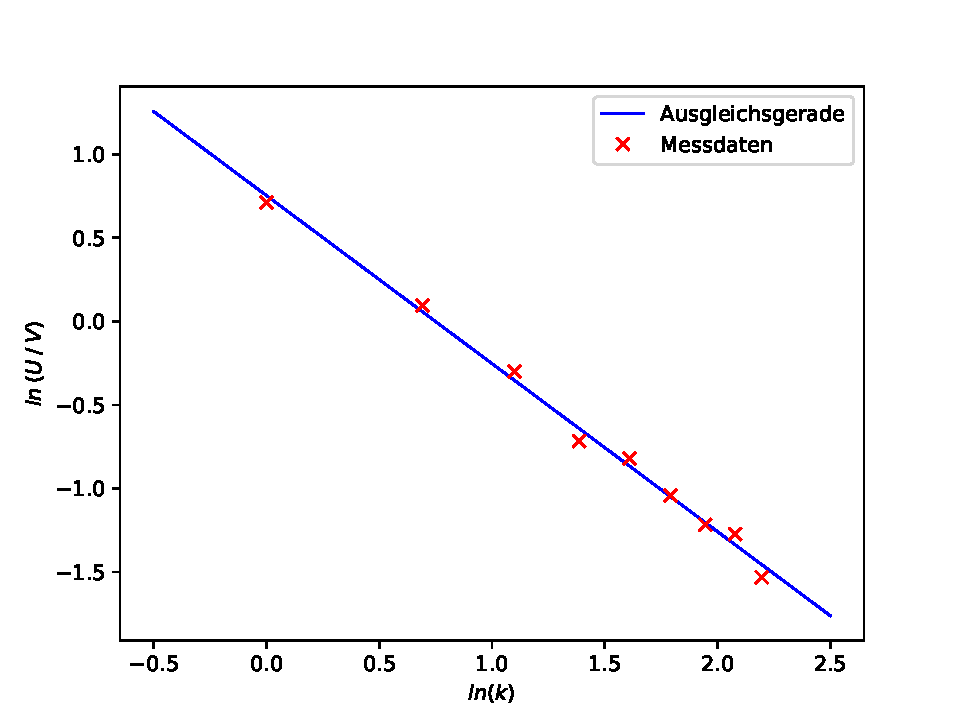
\includegraphics[scale=1.0]{content/plot1.pdf}
    \caption{Messwerte und lineare Regression für die Messwerte der Sägezahnspannung}
    \label{fig:Säge}
\end{figure}

Die Lineare Regression, die mittels python durchgeführt wurde, ergibt die Tangentenparameter:

\begin{align*}
    a_\text{S} &= \SI{-1.0052 \pm 0.0286}{}, \\
    b_\text{S} &= \SI{0.7523 \pm 0.0451}{}.
\end{align*}

Somit liegt die Abweichung zwischen $a_\text{S}$ und $a_\text{S,theo} = \SI{-1}{}$ bei $\SI{0.52}{\percent}$ und
nach Formel \eqref{eqn:Spannung} ist zu erkennen, dass die Fourierkoeffizienten der Sägezahnspannung in etwa
proportional zu $\frac{1}{k}$ abfallen, wie bereits vorbereitend berechnet.
\\
Für die Rechtecksspannung sind die Messdaten in Tabelle \ref{tab:Messdaten2} aufgelistet.

\begin{table}[H]
    \centering
    \caption{Messdaten und deren Logarithmen der Rechtecksspannung}
    \label{tab:Messdaten2}
    \sisetup{table-format=2.1}
    \begin{tabular}{c c c c}
    \toprule
    $k$ & $\text{ln} (k)$ & $U \,/\, \si{\volt}$ & $\text{ln}(U \, \cdot \, \frac{1}{\si{\volt}})$ \\
    \midrule
    1 & 0,000 & 4,000 &  1,389 \\
    3 & 1,099 & 1,440 &  0,365 \\
    5 & 1,609 & 0,860 & -0,151 \\
    7 & 1,946 & 0,580 & -0,545 \\
    9 & 2,197 & 0,420 & -0,868 \\
   11 & 2,398 & 0,384 & -0,957 \\
   13 & 2,565 & 0,344 & -1,067 \\
   15 & 2,708 & 0,280 & -1,273 \\
   17 & 2,833 & 0,224 & -1,496 \\
   19 & 2,944 & 0,216 & -1,532 \\
    \bottomrule
    \end{tabular}
\end{table} 

Diese werden in Abbildung \ref{fig:Recht} gegeneinander aufgetragen. 

\begin{figure}[H]
    \centering
    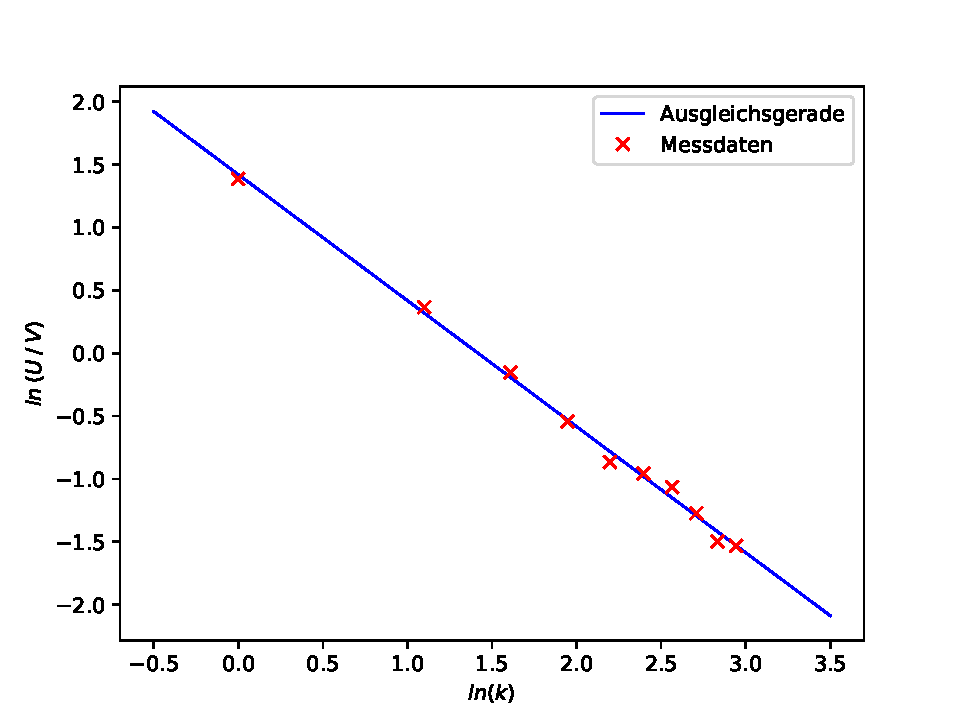
\includegraphics[scale=1.0]{content/plot2.pdf}
    \caption{Messwerte und lineare Regression für die Messwerte der Rechtecksspannung}
    \label{fig:Recht}
\end{figure}

Es ergeben sich die Regressionsparameter:

\begin{align*}
    a_\text{R} &= \SI{-1.0021 \pm 0.0209}{}, \\
    b_\text{R} &= \SI{1.4205 \pm 0.0462}{}.
\end{align*}

Somit liegt die Abweichung zwischen $a_\text{R}$ und $a_\text{R,theo} = \SI{-1}{}$ bei $\SI{0.21}{\percent}$ und
nach Formel \eqref{eqn:Spannung} ist zu erkennen, dass die Fourierkoeffizienten der Rechtecksspannung in etwa
proportional zu $\frac{1}{k}$ abfallen, wie bereits prognostiziert.
\\
\newpage
Für die Dreiecksspannung sind die Messdaten in Tabelle \ref{tab:Messdaten3} aufgelistet.


\begin{table}[H]
    \centering
    \caption{Messdaten und deren Logarithmen der Dreiecksspannung}
    \label{tab:Messdaten3}
    \sisetup{table-format=2.1}
    \begin{tabular}{c c c c}
    \toprule
    $k$ & $\text{ln} (k)$ & $U \,/\, \si{\volt}$ & $\text{ln}(U \,\cdot\, \frac{1}{\si{\volt}})$ \\
    \midrule
     1 & 0,000 & 2,560 &  0,940 \\
     3 & 1,099 & 0,312 & -1,165 \\
     5 & 1,609 & 0,112 & -2,189 \\
     7 & 1,946 & 0,056 & -2,882 \\
     9 & 2,197 & 0,036 & -3,324 \\
    11 & 2,398 & 0,023 & -3,772 \\
    13 & 2,565 & 0,017 & -4,075 \\
    \bottomrule
    \end{tabular}
\end{table} 

Diese sind in Abbildung \ref{fig:Drei} gegeneinander aufgetragen. 

\begin{figure}[H]
    \centering
    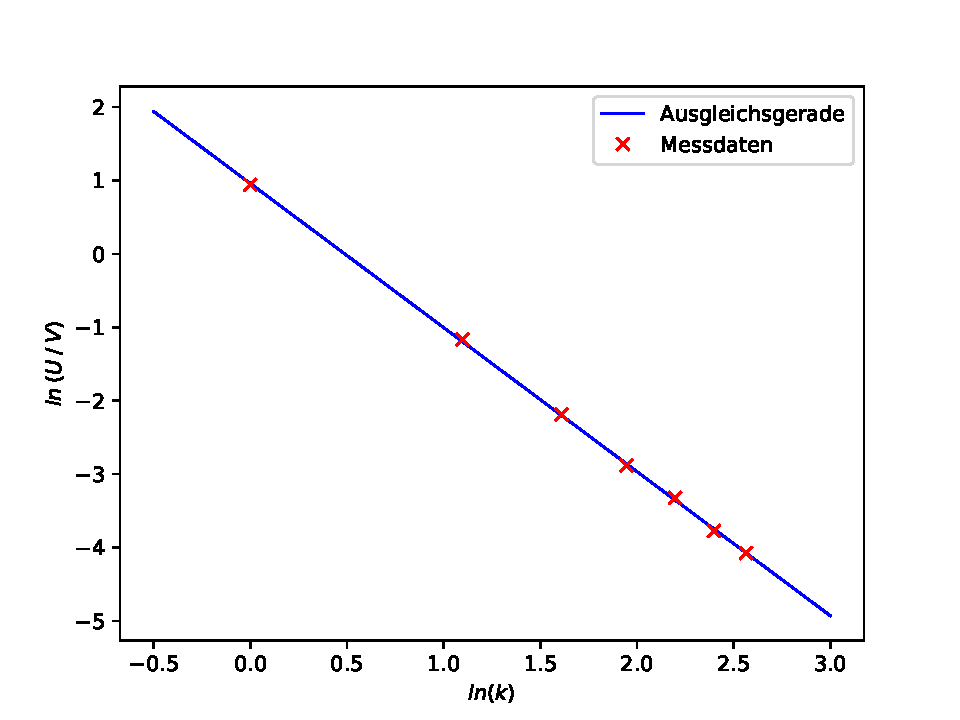
\includegraphics[scale=1.0]{content/plot3.pdf}
    \caption{Messwerte und lineare Regression für die Messwerte der Dreiecksspannung}
    \label{fig:Drei}
\end{figure}

Es ergeben sich die Regressionsparameter:

\begin{align*}
    a_\text{D} &= \SI{-1.9681 \pm 0.0121}{}, \\
    b_\text{D} &= \SI{0.9585 \pm 0.0227}{}.
\end{align*}

Somit liegt die Abweichung zwischen $a_\text{R}$ und $a_\text{R,theo} = \SI{-2}{}$ bei $\SI{1.60}{\percent}$ und
Nach Formel \eqref{eqn:Spannung} ist zu erkennen, dass die Fourierkoeffizienten der Dreiecksspannung in etwa
proportional zu $\frac{1}{k^2}$ abfallen, wie bereits in der in der Vorbereitung berechnet.


\subsection{Fourier-Synthese}

Im zweiten Versuchsteil wird gezeigt, dass sich die verschiedenen Spannungsfunktionen
durch Superpositionen verschiedener Oberwellen, bzw Fourierkoeffizienten synthetisieren
lassen. Als Grundlage dessen dienen theoretische Vorberechnungen der jeweiligen
Fourier-Reihen, nach Formel \eqref{eqn:Entwicklung}, und der in diese eingesetzten
Fourierkoeffizienten $a_k$ und $b_k$.

Für die ungerade Sägezahnspannung sind die Fourierkoeffizienten:

\begin{align*}
    a_\text{k} &= 0 \\
    b_\text{k} &= - \frac{1}{2k} + \frac{1}{k}
\end{align*}

Diese ergeben in Formel \eqref{eqn:Entwicklung} eingesetzt die Fourier-Reihe
der Sägezahnspannung, die in Abbbildung \ref{fig:Theo1} dargestellt ist.

\begin{figure}[H]
    \centering
    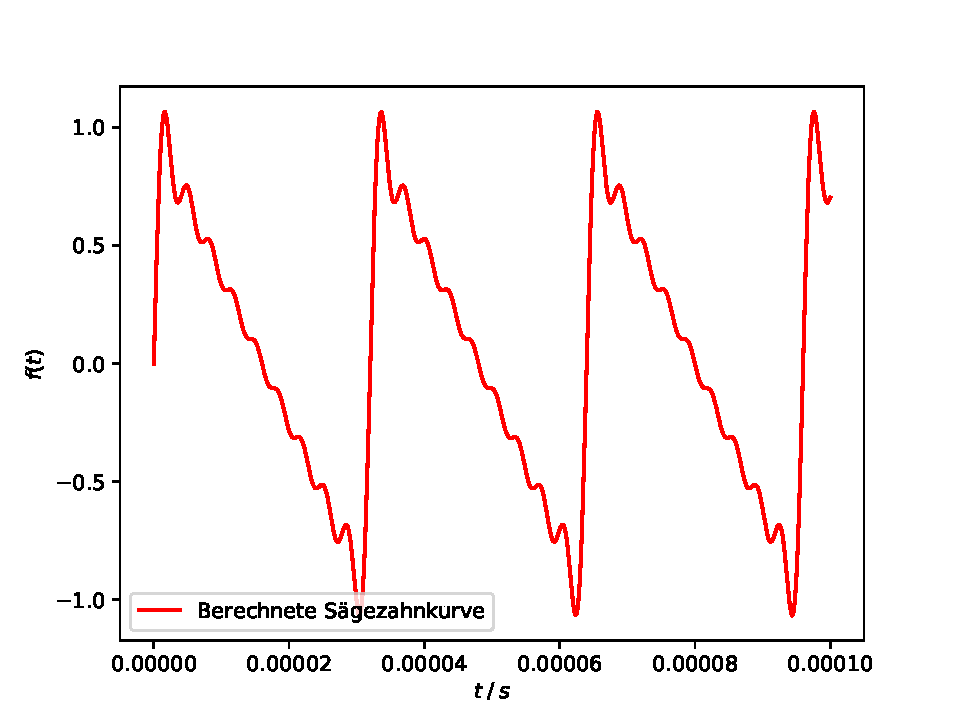
\includegraphics[scale = 0.6]{content/plot4.pdf}
    \caption{Theoretische Sägezahnfunktion}
    \label{fig:Theo1}
\end{figure}

Experimentell werden die Fourierkoeffizienten bzw. Oberwellenamplituden möglichst mit dem
Proportionalitätsfaktor $\frac{1}{k}$ abfallend eingestellt, wie in Tabelle \ref{tab:Messdaten4}
dargestellt. Dabei bezeichnen $U_\text{theo}$ die theoretisch einzustellenden und $U$ die
tatsächlich eingestellten Spannungamplituden. $\symup{\Delta}U$ bezeichnet die Abweichung der
beiden Werte voneinander.

\begin{table}[H]
    \centering
    \caption{Einstellungen der Oberwellenamplituden für eine Sägezahnspannung}
    \label{tab:Messdaten4}
    \sisetup{table-format=2.1}
    \begin{tabular}{c c c c}
    \toprule
    $k$ & $U \,/\, \si{\volt}$ & $U_\text{theo} \,/\, \si{\volt}$ & $\symup{\Delta}U \,/\, \si{\percent})$ \\
    \midrule
    1 & 0,633 & 0,633 & 0,00 \\
    2 & 0,316 & 0,317 & 0,32 \\
    3 & 0,211 & 0,211 & 0,00 \\
    4 & 0,157 & 0,158 & 0,63 \\
    5 & 0,126 & 0,127 & 0,79 \\
    6 & 0,106 & 0,106 & 0,00 \\
    7 & 0,089 & 0,090 & 1,11 \\
    8 & 0,078 & 0,079 & 1,27 \\
    9 & 0,070 & 0,070 & 0,00 \\
   10 & 0,063 & 0,063 & 0,00 \\
    \bottomrule
    \end{tabular}
\end{table}

Daraus ergibt sich die Sägezahnspannung, welche in Abbildung \ref{fig:Ex1}
dargestellt ist.

\begin{figure}[H]
    \centering
    \includegraphics[scale = 0.7]{content/saege.jpg}
    \caption{Experimentell synthetisierte Sägezahnspannung}
    \label{fig:Ex1}
\end{figure}

Für die ungerade Rechtecksspannung lauten die Fourierkoeffizienten:

\begin{align*}
    a_\text{k} &= 0 \\
    b_\text{k} &= 
        \begin{cases} 
            0, \text{ für k gerade} \\ \frac{4}{\pi k}, \text{ für k ungerade}
        \end{cases}
\end{align*}

Diese ergeben in Formel \eqref{eqn:Entwicklung} eingesetzt die Fourier-Reihe
der Rechtecksspannung, die in Abbbildung \ref{fig:Theo2}  dargestellt ist.

\begin{figure}[H]
    \centering
    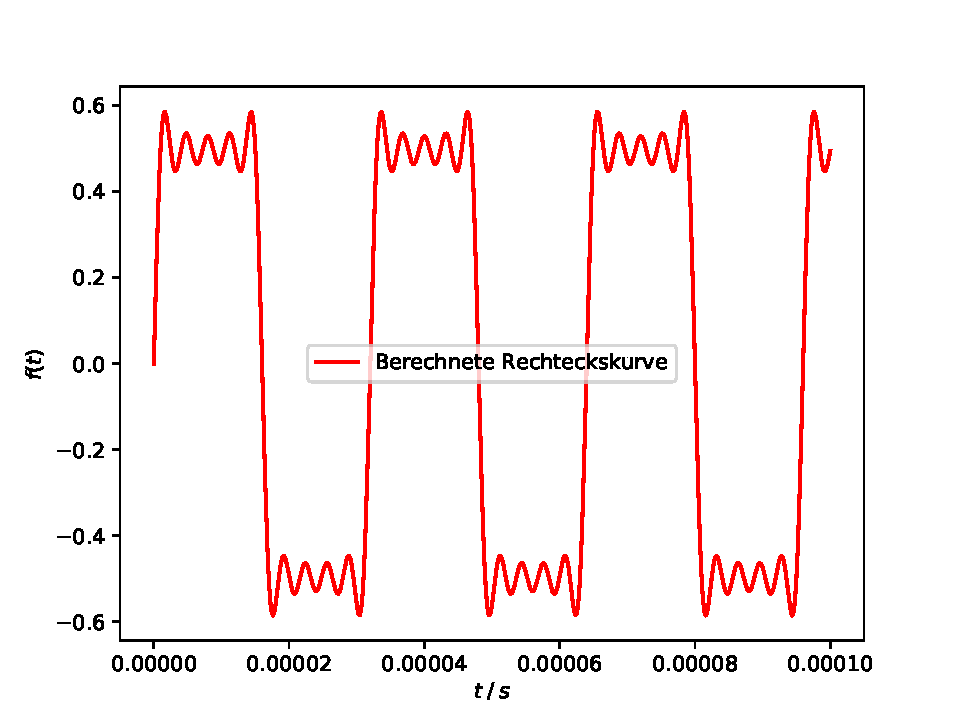
\includegraphics[scale = 0.6]{content/plot5.pdf}
    \caption{Theoretische Rechtecksfunktion}
    \label{fig:Theo2}
\end{figure}

Die Fourierkoeffizienten der Rechtecksspannung werden analog zu denen der Sägezahnspannung
eingestellt, wie in Tabelle \ref{tab:Messdaten5} dargestellt. 

\begin{table}[H]
    \centering
    \caption{Einstellungen der Oberwellenamplituden für eine Rechtecksspannung}
    \label{tab:Messdaten5}
    \sisetup{table-format=2.1}
    \begin{tabular}{c c c c}
    \toprule
    $k$ & $U \,/\, \si{\volt}$ & $U_\text{theo} \,/\, \si{\volt}$ & $\symup{\Delta}U \,/\, \si{\percent})$ \\
    \midrule
     1 & 0,633 & 0,633 & 0,00 \\
     2 & 0,000 & 0,000 & 0,00 \\
     3 & 0,211 & 0,211 & 0,00 \\
     4 & 0,000 & 0,000 & 0,00 \\
     5 & 0,126 & 0,127 & 0,79 \\
     6 & 0,000 & 0,000 & 0,00 \\
     7 & 0,089 & 0,090 & 1,11 \\
     8 & 0,000 & 0,000 & 0,00 \\
     9 & 0,070 & 0,070 & 0,00 \\
    10 & 0,000 & 0,000 & 0,00 \\
    \bottomrule
    \end{tabular}
\end{table}

Daraus ergibt sich die Rechtecksspannung, welche in Abbildung \ref{fig:Ex2}
dargestellt ist.

\begin{figure}[H]
    \centering
    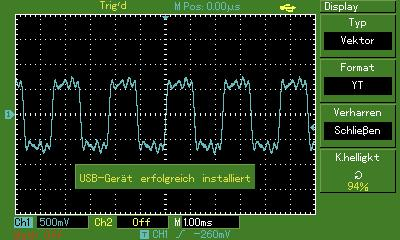
\includegraphics[scale=0.7]{content/recht.jpg}
    \caption{Experimentell synthetisierte Rechtecksspannung}
    \label{fig:Ex2}
\end{figure}


Für die gerade Dreiecksspannung lauten die Fourierkoeffizienten:

\begin{align*}
    a_\text{k} &= 0 
        \begin{cases} 
            0, \text{ für k gerade} \\ \frac{8}{\pi^2 k^2}, \text{ für k ungerade}
        \end{cases} \\
    b_\text{k} &= 0
\end{align*}

Diese ergeben in Formel \eqref{eqn:Entwicklung} eingesetzt die Fourier-Reihe
der Dreiecksspannung, die in Abbbildung \ref{fig:Theo3}  dargestellt ist.

\begin{figure}[H]
    \centering
    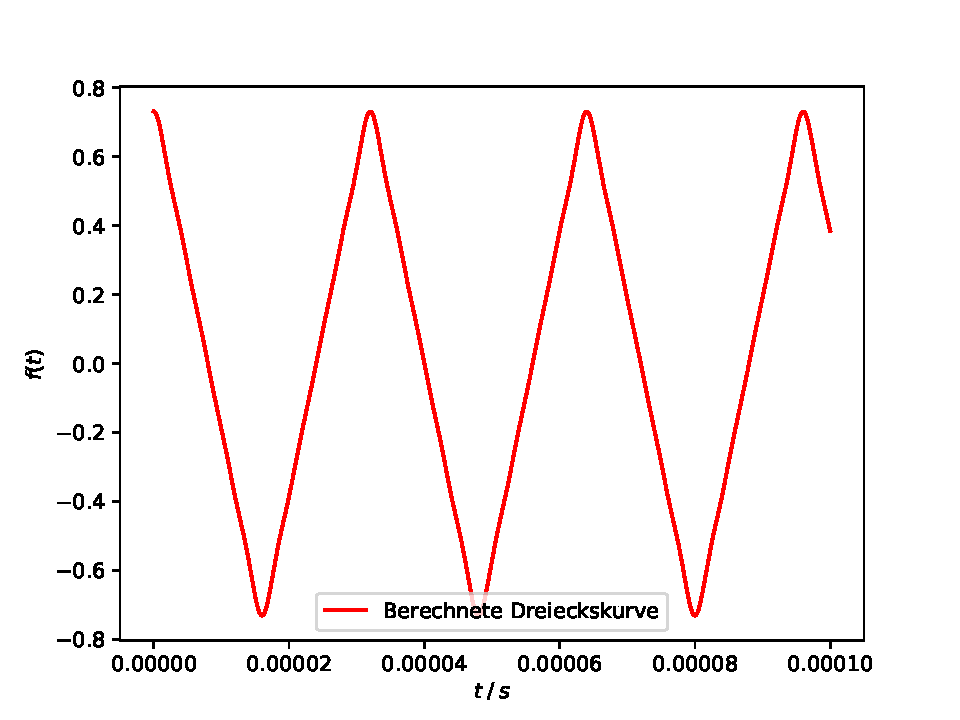
\includegraphics[scale = 0.6]{content/plot6.pdf}
    \caption{Theoretische Dreiecksfunktion}
    \label{fig:Theo3}
\end{figure}

Die Fourierkoeffizienten der Dreiecksspannungen werden im Gegensatz zu denen
der vorherigen mit einem Abfall proportional zu $\frac{1}{k^2}$ eingestellt,
wie in Tabelle \ref{tab:Messdaten6} dargestellt. Die abgebildeten
Größen ergeben sich analog zu den Tabellen der anderen beiden Spannungen.

\begin{table}[H]
    \centering
    \caption{Einstellungen der Oberwellenamplituden für eine Dreiecksspannung}
    \label{tab:Messdaten6}
    \sisetup{table-format=2.1}
    \begin{tabular}{c c c c}
    \toprule
    $k$ & $U \,/\, \si{\volt}$ & $U_\text{theo} \,/\, \si{\volt}$ & $\symup{\Delta}U \,/\, \si{\percent})$ \\
    \midrule
    1 & 0,617 & 0,617 & 0,00 \\
    2 & 0,000 & 0,000 & 0,00 \\
    3 & 0,068 & 0,069 & 1,45 \\
    4 & 0,000 & 0,000 & 0,00 \\
    5 & 0,025 & 0,025 & 0,00 \\
    6 & 0,000 & 0,000 & 0,00 \\
    7 & 0,013 & 0,013 & 0,00 \\
    8 & 0,000 & 0,000 & 0,00 \\
    9 & 0,008 & 0,008 & 0,00 \\
    \bottomrule
    \end{tabular}
\end{table}

Es ergibt sich schließlich die Dreiecksspannung, welche in Abbildung \ref{fig:Ex3}
dargestellt ist.

\begin{figure}[H]
    \centering
    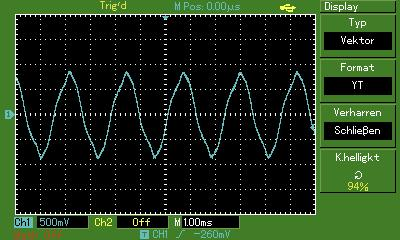
\includegraphics[scale=0.7]{content/sinus.jpg}
    \caption{Experimentell synthetisierte Dreiecksspannung}
    \label{fig:Ex3}
\end{figure}




